We demonstrate the correlation effect of the reconstructed kSZ signal in Fig.\ref{fig:powermomen15}. The upper panel shows the powerspectrum of orginal kSZ signal $P_{kSZ}$, reconstructed kSZ signal from 21cm intensity mapping $P_{21cm}$ and the cross powerspectrum of this two field $P_{cross}$; 
and the lower panel demonstrates the correlation r between reconstructed kSZ signal $\hat\Theta$ and the orginal kSZ signal $\Theta$. 
As we can see, we have a stable 0.3 correlation from $l\sim 100$ to $l\sim 2000$, which indicates a detectable signal in real observations.

\begin{figure}[tbp]
	\begin{center}
		\includegraphics[width=0.48\textwidth,height=0.52\textheight]{powermomen15.eps}
	\end{center}
	\vspace{-0.7cm}
	\caption{(Top) the powerspectrum of orginal kSZ signal $P_{kSZ}$, reconstructed kSZ signal from 21cm intensity mapping $P_{21cm}$ and the cross powerspectrum of this two field $P_{cross}$; 
(Bottom) the correlation r between reconstructed kSZ signal $\hat\Theta$ and the orginal kSZ signal $\Theta$.} 
\label{fig:powermomen15}
\end{figure}


